%%%%%%%%%%%%%%%%%%%%%%%%%%%%%%%%%%%%%%%%%%%%%%%%%%%%%%%%%%%%%%%%%%%%%%%%%%%%%%%
% intro.tex: Introduction to the thesis
%%%%%%%%%%%%%%%%%%%%%%%%%%%%%%%%%%%%%%%%%%%%%%%%%%%%%%%%%%%%%%%%%%%%%%%%%%%%%%%%
\chapter{Introduction}
\label{intro_chapter}
%%%%%%%%%%%%%%%%%%%%%%%%%%%%%%%%%%%%%%%%%%%%%%%%%%%%%%%%%%%%%%%%%%%%%%%%%%%%%%%%
\section{Geometric and functional analytic methods in dynamical systems}
Problems in Dynamical systems deals primarily with systems of ordinary differential equations (ODEs). In most introductory graduate classes about ODEs, two perspectives are often presented to the students: on one hand, we have the analysis approaches. The most obvious example is the proof of the basic existence and uniqueness theorem for a general $n-$dimensional system of ODEs, where one usually sees Banach's fixed point theorem for the first time. On the other hand, we have the geometric approaches that qualitatively describes the behavior of system of ODEs. One would think of phase-plane analysis, and perhaps the theory of invariant manifolds which proves to be essential in long-time behavior questions.

While both approaches are important, this paper will focus on the first prospective for two main reasons. First, for problems beyond the traditional ODE-setting, it is easier to recast the problem in a functional analytic framework and extend known result. Second, we found that even in problems usually dealt by the geometric approaches, it is possible to give a conceptually cleaner and easier-to-follow proof when reinterpreting the problem using functional analysis. We shall demonstrate these two points via two examples. In the first example, we show how to extend results about radially symmetric solutions bifurcating from systems of partial differential equations to nonlocally coupled systems by appropriately set it up as a fixed point problem. In the second example, we revisit a problem from singular perturbation theory that is solved using the geometric blow-up method, and show that we can achieve the same result again by rewriting it as an appropriate fixed point problem with multiple parts.

\section{Nonlocal spikes}\label{s:1}
Much of the success of modeling has been based on infinitesimal descriptions of physical laws, leading to differential and partial differential equations as models for physical processes. However, many physical interactions are inherently nonlocal, at least at a coarser modeling level, leading to nonlocal spatial coupling, as well as dependence of time evolution on history. From a dynamical systems point of view, a natural question in this context is in how far nonlocally coupled equations may behave qualitatively differently from locally coupled problems. As usual, one can approach this question from several vantage points, striving in particular to point to phenomena where nonlocality generates new phenomena, or delineate situations where nonlocal and local equations behave in analogous fashions. Our contribution here is mainly towards the latter aspect, showing that local bifurcations in nonlocal systems produce coherent structures completely analogous to local systems. We will however also comment on phenomena that are qualitatively different as a result of nonlocality. 

In the first part of this paper, we will focus on a fairly simple model problem, stationary solutions to nonlocally coupled systems, solving
\begin{equation} \label{system}
U+\K\ast U = \Nl(U;\mu) ,
\end{equation}
where $U=U(x)\in\R^k$, $x\in\R^n$, $\K\ast U$ stands for matrix convolution,
\[
(\K\ast U(x))_i = \sum_{j=1}^m \int_{\R^n} \K_{i,j}(x-y)U_j(y)dy, \hspace{0.2in} 1\le i\le k,
\]
and $\Nl(U;\mu)$ encodes nonlinear terms which depend on a parameter $\mu\sim 0$. 

We are interested in the existence of spatially localized solutions $U(x)\to U_\infty$, $|x|\to\infty$ in the  prototypical setting of a transcritical bifurcation of spatially constant solutions $U(x)\equiv m$. 

In the remainder of the introduction for the first part, we shall first provide some background and motivation for this kind of question, Section \ref{s:mot}, and then give precise assumptions and results in Sections \ref{s:set} and \ref{s:res}. We collect some standard notation used throughout the first part at the end. 


\subsection{Motivation}\label{s:mot}

\paragraph{Applications with nonlocal coupling.} Nonlocal coupling has been suggested as a more appropriate modeling assumptions in fields all across the sciences. Prominent examples are nonlocal dispersal of plant seeds in ecology \cite{plantdisp}, fractional powers of the Laplacian as limits of random walks with Levy jumps \cite{levy}, models for neural fields \cite{neuralfieldrev}, nonlocal interactions in models for Bose-Einstein condensates \cite{bose}, kinetic equations for interacting particles \cite{swarmingrev}, shallow water-wave models \cite{waterwave}, or material science \cite{matsci}. In many of these models, one is interested in spatially localized or front-like solutions, stationary, periodic,  or  propagating in time,  which we will here refer to collectively as  coherent structures. Such solutions are usually found through a traveling-wave ansatz, thus eliminating or compactifying time dependence.  In some special situations, Many of the above examples can thereby be reduced to problems of the type \eqref{system}, and we will give details for some cases in Section \ref{s:app}. 

Arguably, the most powerful results for existence and stability of coherent structures rely on formulating the existence problem as an ordinary differential equation, a method sometimes referred to as ``spatial dynamics'' \cite{sandtw} --- for locally coupled equations, in essentially one-dimensional geometries such as the real line, cylinders $\R\times\Omega$, or with radial symmetry. We will briefly overview such results from our perspective here and discuss in how far they generalize to nonlocally coupled equations, before turning to our contribution in more detail in Sections \ref{s:set}--\ref{s:res}. 


\paragraph{Local coupling --- results.} 
Replacing nonlocal coupling by diffusive coupling, say $D\Delta U$, with $D$ positive, diagonal, we can consider  the elliptic system 
\begin{equation}\label{e:rd}
\Delta U + \Nl(U;\mu)=0,
\end{equation}
with $x\in\R^n$. In the simplest case of $n=1$, one can study the resulting ordinary differential equation 
\begin{equation*}
U_x=V,\qquad 
V_x=-\Nl(U;\mu),
\end{equation*}
using dynamical systems methods such as center-manifold reduction and normal form transformations, thus leading to nearly universal predictions for bifurcations of coherent structures. In addition to existence results, such methods also allow one to state rather general uniqueness and non-existence results. In higher space dimensions, $n>1$, such reduction techniques are not known to be applicable, except for the context of radial symmetry, which allows one to formulate the existence problem as a dynamical system in the radial variable $r$, 
\begin{equation*}
U_r=V,\qquad
V_r=-\frac{n-1}{r}V-\Nl(U;\mu).
\end{equation*}
Slightly adapted center manifold and normal form theory again leads to near-universal classifications of small-amplitude coherent structures; see \cite{Srad} for a comprehensive exposition of these techniques and \cite{harioo} for background on center manifolds and normal forms. 

In the simplest case of a transcritical bifurcation in the nonlinearity, with suitable additional assumptions on the linear part, one finds a reduced equation on the center manifold of the form 
\begin{align*}
u_x&=v+\rmO\left(|\mu|(|u|+|v|)+u^2+v^2\right),\\
v_x&=\mu u - u^2 + \rmO\left(v^2+(|u|+|v|)(\mu^2+u^2+v^2)\right),
\end{align*}
which at leading order, after scaling, reduces to 
\begin{equation}\label{e:tc}
u_{xx}- u + u^2=0,
\end{equation}
with an explicit nontrivial localized solution $u(x)\to 0,\ |x|\to\infty$. Using reversibility $x\mapsto -x$ one then readily shows persistence of this solution at higher order. Exploiting the characterization of center manifolds, one also obtains non-existence of other localized solutions and, in fact, a complete characterization of small bounded solutions. 

The results in \cite{Srad} extend this machinery to radially symmetric solutions in higher space dimension, leading to a leading order equation of the form 
\[
u_{rr}+\frac{n-1}{r}u_r - u + u^2=0.
\]
This type of results is also available for Turing and Hopf bifurcations \cite{Srad}. It is however not immediately applicable to the type of nonlocally coupled equations described above, with recent progress that we shall describe next. 


\paragraph{Nonlocal coupling --- center manifolds.} Going back to \eqref{system}, we can in general not find an obvious formulation as a dynamical system, with the notable exception of convolution kernels with a rational Fourier transform. Consider for instance $\K(x)=\frac{1}{2}\rme^{-|x|}$, $x\in\R$, with Fourier transform $\hat{\K}(\xi)=(1+\xi^2)^{-1}$, for which we can formally write \eqref{system} as $(\id -\Delta)^{-1}U+\Nl(U;\mu)=0$, which in turn is equivalent to 
\begin{align*}
-U+W+\Nl(U;\mu)&=0,\\
W-\Delta W &=U.
\end{align*}
Under suitable assumptions, equivalent to stability assumptions made in \cite{Srad}, one can solve the first equation for $U=\Psi(W;\mu)$ and insert into the second equation, thus obtaining a local equation for $W$, 
\[
\Delta W -W + \Psi(W;\mu)=0,
\]
which is amenable to the methods from \cite{Srad}. 

The restriction to kernels with rational Fourier transform is clearly restrictive, excluding for instance Gaussians, and one naturally wonders if similar results hold outside of this class. The more recent results in \cite{FScmfd} answer this question in the affirmative, for $x\in\R$ and $\K,\K'$ exponentially localized, such that $\hat{\K}$ is analytic in a strip of the complex plane $|\Re\xi|<\eta$. 

Some smoothness of $\K$ appears to be necessary, as the counter example of $\K=\frac{1}{2}(\delta_{-1}+\delta_{1})$ shows, which produces a simple iteration 
\[
\frac{1}{2}\left(U(x+1)-2U(x)+U(x-1)\right)+\Nl(U;\mu)=0,
\]
with completely uncorrelated solutions on lattices $x\in x_0+\Z$. A finite-dimensional reduction to an ordinary differential equation here does not seem possible. 

Also, exponential localization appears to be necessary. Algebraically localized kernels typically yield algebraically localized profiles but solutions of reduced differential equations would typically converge exponentially. Nevertheless, our results remove the assumption of exponential localization, at the expense of lacking a general uniqueness argument. We still reduce to the simple ordinary differential equation \eqref{e:tc} or its higher-dimensional analogue, with exponentially localized solutions, and find weaker far-field decay only at higher order in the bifurcation parameter $\mu$.

\subsection{Setup --- linear nonlocal diffusive coupling and local bifurcations of spatially constant states}\label{s:set}
Within the context described in the previous section, we are now ready to state our main assumptions and results. We start with assumptions on the linear part, keeping in mind that the nonlinearity will be assumed to be of quadratic order in $U,\mu$, then turn to assumptions on the nonlinearity, before stating our main result. 

\paragraph{Linear diffusive coupling.}

Let $I_k$ denote the identity matrix of size $k$ and consider the linearized operator $I_k + \K*$. 

\begin{Hypothesis}{(L)}We assume that  $\K$ satisfies the following properties:
\begin{enumerate}
\item \emph{localization:  }$\K$ has finite moments of order 2, that is, 
\[\K(x),\, |x|^2\K(x) \in L^1(\R^n,\R^{k\times k});\]
\item \emph{symmetry: } $\K(x)=\K(\gamma x)$ for all $x\in\R^n$ and all $\gamma \in \Gamma\subset \mathbf{O}(n)$, a subgroup of the orthogonal matrices with 
\[
\mathrm{Fix}\, \Gamma=\left\{x\mid\gamma x=x, \mbox{ for all } \gamma\in\Gamma\right\}=\{0\};
\]
\item \emph{minimal nullspace: } $\Ns(I_k+\int\K)=\mathrm{span}\, {\e}$ for some  $ 0\neq {\e}\in \R^k$; we then choose ${\e}^*$ such that   $\Ns(I_k+\int\K^T)=\mathrm{span}\, {\e}^*$;
\item \emph{nondegenerate second moments:}  the matrix of projected second moments $S$ with entries 
\[
S_{ij}=\int x_ix_j \langle{\e}^*,\K(x) {\e}\rangle\rmd x,
\]
is positive definite;
\item \emph{invertibility for nonzero wavenumbers: } $I_k+ \int \rme^{\rmi \langle \xi,x\rangle}\K(x)\rmd x$ is invertible for all $\xi\neq 0$. 
\end{enumerate}
\end{Hypothesis}
The assumption on positive definiteness can be readily replaced by negative definiteness, simply multiplying the equation by $-1$. 
Note that first moments, $\int x\K(x)\rmd x$ vanish, since
\begin{equation}\label{e:1st}
\int x \K(x)\rmd x=\int x K(\gamma x)\rmd x= \gamma^{-1}\int y \K(y)\rmd y,
\end{equation}
for all $\gamma\in \Gamma$, hence $\int x \K(x)\rmd x=0$ since $\Gamma$ fixes the origin, only. In fact, this is the primary reason for us to require the symmetry mentioned here. Nonvanishing first moments correspond to an effective directional transport which would need to be compensated by a drift term $c\cdot \nabla U$, say, in order to find coherent structures. 

Typical examples of symmetry groups $\Gamma$ are $\Gamma=\mathbf{O}(n)$, $\Gamma=\{\mathrm{id},-\mathrm{id}\}$ or the group generated by reflections at hyperplanes, $x_j\mapsto -x_j$. 

\begin{Remark}[normalizing second moments]\label{r:rs} There exists a coordinate change $x=T_0y$ such that the transformed kernel $\tilde{\K}(y):=|\mathrm{det}\,T_0|\K(T_0y)$ satisfies
\[
\tilde{S}_{ij}=\int x_ix_j\langle {\e}^*,\tilde{\K}(x) {\e}\rangle\rmd x=2\delta_{ij}.
\]
Indeed, let $\lambda_i$, $i=1,\ldots,k$ be the eigenvalues of $S$ and $P_i$ be the associated spectral projections. Define
\[
T_0 = \sum_{i} \sqrt{2}(\lambda_i)^{-1/2} P_i, \hspace{0.5in} \tilde{M}(y) = \langle {\e}^*, \tilde{K}(x){\e} \rangle ,\hspace{0.5in}  {M}(y) = \langle {\e}^*, {K}(x){\e} \rangle .
\]
Then
\begin{align*}
\tilde{S}_{ij} &= \int x_ix_j \tilde{M}(x) \rmd x 
= \int (T_0^{-1}y)_i(T_0^{-1}y)_jM(y)\rmd y
= \sum_{k,l}T^{-1}_{0,ik}T^{-1}_{0,jl}S_{kl}
= T_0^{-1}S(T_0^{-1})^{T}\\
&=\left(\sum_\ell \sqrt{2}\lambda_\ell^{-1/2}P_\ell\right)\left(\sum_m \lambda_m P_m\right)\left(\sum_k \sqrt{2}\lambda_k^{-1/2}P_k\right)=2\sum P_\ell=2I_k.
\end{align*}
Note that the new kernel $\tilde{\K}$ possesses all the properties assumed for $\K$ in Hypothesis (L). In particular, $\tilde{K}$ is invariant under $\Gamma$. To see this, notice that $S\gamma=\gamma S$ for all $\gamma$, and conclude that $T_0\gamma=\gamma T_0$ since spectral projections commute with $\gamma\in\Gamma$, as well. As a consequence, $\tilde{K}$ is invariant. 
\end{Remark}

The assumptions can also be stated in terms of the associated Fourier determinant $\mathcal{D}$,
\[
\mathcal{D}(\xi):=\det(I_k+\widehat{\K}(\xi)).
\]
One readily finds that $\mathcal{D}$ is of class $\mathscr{C}^2$ by the assumption on second moments, and 
\[
\mathcal{D}(0)=0,\qquad  \mathcal{D}'(0)=0, \qquad  \mathcal{D}''(0)\neq 0.
\]
The characteristic function $\mathcal{D}$ was also used in \cite{FScmfd}, identifying zeros of $\mathcal{D}$ on the real axis with bounded solutions to the linear equation, and, more generally, multiplicities of zeros adding up to the dimension of a reduced center manifold as algebraic multiplicities of a center subspace. In the setup there, $\mathcal{D}$ was analytic, allowing readily for characterizing the multiplicity of roots. We here assume just enough regularity, $\mathscr{C}^2$ to make sense of a ``double root'' of $\mathcal{D}$.

\begin{Remark}[generalizing linear assumptions]\label{r:gl}
Most examples of nonlinear problems would involve a nontrivial pointwise linear part, say, $AU+\K*U$. One quickly sees that these and more general terms should be viewed as less smooth, namely Dirac-$\delta$ contributions to the matrix kernel. Whenever this principle part, say, the matrix $A$, is invertible, the system can be readily put into our form by applying $A^{-1}$. On the other hand, when this principal part possesses a kernel, our assumption of invertibility for nonzero wavenumbers would be violated asymptotically, for $\ell\to\infty$. Bifurcation solutions in such situations are not necessarily smooth. 
\end{Remark}

%
Yet a different interpretation would refer to the spectrum of the linear part $I_k + \K*$, given by the set of $\lambda$ for which $I_k + \K*-\lambda I_k$ is not invertible, or, equivalently, the  closure of the set of $\lambda$ such that $\det(I_k+\widehat{\K}(\xi)-\lambda I_k)= 0$ for some $\xi\in\R$. Clearly, $\lambda=0$ is in the spectrum, choosing $\xi=0$. Also, $\lambda=0$ is minimal in multiplicity in the sense that it is an eigenvalue only for $\xi=0$, and its geometric multiplicity at $\xi=0$ is minimal. Assuming that, in addition, $\lambda=0$ is algebraically simple, one readily finds that the continuation of $\lambda$ as an eigenvalue in $\xi$ is quadratic, $\lambda= \langle \mathcal{S}\xi,\xi\rangle+\ldots$, with definite symmetric matrix  $\mathcal{S}$. Such spectral information can in general be converted into heat decay estimates for $U_t=-U+\K*U$ \cite{heatnl}.


\paragraph{Transcritical bifurcation for spatially constant solutions.}
As mentioned, we assume the presence of a simple transcritical bifurcation in the nonlinearity $\Nl$. The assumptions that follow are generic and necessary for a non-degenerate bifurcation scenario; see for example \cite{chowhale}.  They single out relevant terms in systems of equations that lead to bifurcations as in the simple scalar example $\Nl(u;\mu)=\mu u - u^2$. 
 
\begin{Hypothesis} {(TC)} We assume that $\Nl=\Nl(U;\mu):\R^k \times \R \to \R^k $ satisfies the following conditions:
\begin{enumerate}
\item 
\emph{smoothness: }
$\mathscr{C}^{K}(\R^k \times \R; \R^k)$, $K=1+\ell+2$;
\item \emph{trivial solution: } $\Nl(0;\mu) = 0$ for all $\mu$;
\item \emph{criticality:} $D_U\Nl(0;0)=0$;
\item \emph{generic linear unfolding:  }
\begin{equation}
\alpha := \langle D_{\mu,U} \Nl(0;0){\e}, {\e}^*\rangle \neq 0; \label{muvCoe}\end{equation}
\item \emph{generic nonlinearity: } 
\begin{equation}
\beta := \frac{1}{2}\langle D_{U,U} \Nl(0;0)[{\e},{\e}], {\e}^*\rangle \neq 0.  \label{QuadCoe}
\end{equation}
\end{enumerate}
\end{Hypothesis}

Smoothness assumptions ensure that the superposition operator $U(\cdot) \mapsto \Nl(U(\cdot);\mu)$ defined by $\Nl$ is of class $\mathscr{C}^1$ as a map on $H^\ell(\R^n,\R^k)$; see for instance \cite{runst1996sobolev}.
%\footnote{should we make this somewhat sharper, something like $C^{2+\ell}$?}

The choice of a transcritical setup here is for convenience and other elementary bifurcations can be treated in a similar fashion. A saddle-node bifurcation, where  $\langle D_{\mu} \Nl(0;0), {\e}^*\rangle \neq 0$,  $\langle D_{U,U} \Nl(0;0)[{\e},{\e}], {\e}^*\rangle \neq 0$, can be transformed into a transcritical bifurcation after subtracting one of the branches, $\tilde{U}=U-U_-(\mu)$ and reparameterizing, say, $\mu=\tilde{\mu}^2$. Also, more general nonlocal dependence of $\Nl$ on $U$ can be allowed. In such a case, Hypothesis (TC) applies to $\Nl$ acting on spatially constant solutions $U$.


\subsection{Bifurcation of spikes --- main result}\label{s:res}

We are now ready to state our main result. As suggested above, we would like to compare our problem to the local problem 
\begin{equation}\label{e:gs}
\Delta u - \alpha\mu u + \beta u^2=0,
\end{equation}
when $U\sim u{\e}$. For $\alpha\mu>0$, this equation possesses localized ground states of the form 
\begin{equation}\label{e:gs00}
u_\mathrm{c}(x;\mu)=-\alpha\beta^{-1}\mu u_*(\sqrt{\alpha\mu} x),
\end{equation}
where $u_*(y)$ is the (positive) ground state to 
\begin{equation}\label{e:gs0}
\Delta u -  u + u^2=0;
\end{equation}
see \cite{gs} for background information on existence of such ground states and their properties. 

\begin{Theorem}[bifurcation of spikes]\label{MainRes} Fix $n<6$ and $\ell>n/2$.  Assume Hypotheses (L) and (TC), and recall the definition of $T_0$ from Remark \ref{r:rs} and $\alpha,\beta$ from \eqref{muvCoe} and \eqref{QuadCoe}.

There then exists a constant $\mu_0>0$ such that for all $0< \alpha\mu<\mu_0$, the nonlocally coupled system \eqref{system} possesses a  family of nontrivial solutions $U_*=U_*(\cdot;\mu) \in H^\ell(\R^n;\R^k)$. Moreover, $U_*(x;\mu)$ is given to leading order through
\begin{equation}\label{expan}
U_*(x;\mu) = {-\alpha\beta^{-1}\mu\left[ u_*(\sqrt{\alpha\mu} \,T_0 x)+w(\sqrt{\alpha\mu} \, x;\mu)\right]{\e} }+ u_{\perp}(x;\mu),
%\qquad  \text{need to correct with } T_0, 
\end{equation}
where 
\begin{itemize}
\item $u_*$ from \eqref{e:gs00} is the  (scalar) radially symmetric ground state to \eqref{e:gs0};
\item the corrector ${w(\sqrt{\alpha\mu} \, x;\mu)}$ satisfies  $\|w(\cdot;\mu)\|_{H^\ell} \to 0$ as $\mu \to 0$;
\item $\langle u_{\perp}(x;\mu),{\e}\rangle=0$, and $\|u_{\perp}\|_{H^\ell} = \rmO(\mu^2)$.
%\footnote{or just $\rmo(\mu)$?}
\end{itemize}
Moreover, $U_*(x;\mu)=U_*(\gamma x;\mu)$ for all $\gamma\in\Gamma$. 
% 
% % 
% 
% If $\frac{1}{2}\langle \widehat{\K}^{''}(0){\e},{\e}^*\rangle := d>0$ and $\alpha>0$, there then exist a positive constant $\mu_0$ sufficiently small, such that \eqref{system} has a family of nontrivial solutions $U_*=U_*(\cdot;\mu) \in H_r^\ell(\R^n;\R^k)$ parametrized by $\mu\in (0,\mu_0) $. 
% 
% Here, $v_{\perp}$ takes value in the complement of ${\e}$, and satisfies $\|v_{\perp}\|_{H^\ell} = \rmO(\mu^2)$ as $\mu \to 0$. $v_\mathrm{c}$ is a scalar function of the form 
% $v_\mathrm{c}(x; \mu)=-\frac{1}{\beta} (\alpha\mu)\left[ v_*(\sqrt{\alpha\mu}x)+w(\sqrt{\alpha\mu}x;\sqrt{\alpha\mu}) \right]$. Here $w(\cdot;\sqrt{\alpha\mu}) \in H^{\ell}_r$ is a corrector function with $\|w(\cdot;\sqrt{\alpha\mu})\|_{H^\ell} \to 0$ as $\mu \to 0$, and $v_*(\cdot)$ is the unique ground state solution to the equation $d\Delta v -u+u^2 =0$, with the condition 
% $v_*(0)>0$ and $\lim_{|x|\to \infty}v_*(x)=0$.
\end{Theorem}

We comment briefly on the scope of this result and outline the main idea of proof. 

We believe that our assumptions are to some extent sharp. The assumption $n < 6$ relates to subcriticality of the nonlinearity in the local, scalar version of our problem,
 $\Delta w - w + w^p = 0.$ Subcriticality of the nonlinearity implies existence of ground states and minimal critical spectrum, and holds for $1 < p < \frac{n+2}{n-2}$
 (\cite[Lem. 13.3]{gs}), or in our case, $n<6$ for $p=2$. Second moments are necessary to define diffusive behavior and obtain the limiting ground state problem. One would suspect that weaker localization, $\hat{\K}\sim |\xi|^{2\nu}$ for $\xi\sim 0$ would lead to reduced problems based on the fractional Laplacian $(-\Delta)^\nu$, with somewhat analogous results. Symmetry of the kernel is necessary to some extent to prevent drift of the resulting spikes. In other words, we find at leading order a manifold of translates of a ground state as solutions. The symmetry condition guarantees that all these solutions persist to higher order as non-degenerate fixed points in the fixed point subspace of the action of $\Gamma$ on profiles. We suspect that alternate assumptions could involve a variational structure in the problem. We will comment on possible drift and the technical ramifications in the discussion section.

%%%%%%%%%%%%%%%%%%%%%%%%%%%%%%%%%%%%%%%%%%%%%%%%%%%%%%%%%%%%%%%%%%%%%%%%%%%%%%%%
\section{Passage through fold}
In the second part of this paper, we study singularly perturbed ordinary differential equations (ODEs) of the form

\begin{align}\label{intro_slow}
\begin{split}
\eps \dot{x} &=  f(x,y;\eps),\\
\dot{y } &=   g(x,y;\eps),   
\end{split}\hspace{0.2in} x\in \mathbb{R}^n, \hspace{0.2in} y \in \mathbb{R}^m, \hspace{0.2in} 0<\eps \ll 1,
\end{align}
where $f$ and $g$ are smooth functions.
\subsection{Background --- geometric singular perturbation theory and blow-up}

The standard way of studying \eqref{intro_slow} is using methods from geometric singular perturbation theory. An brief overview of this theory involves treating \eqref{intro_slow}, which is referred to as the \textit{slow-system}, together with its  equivalent counterpart, the \textit{fast-system}:
\begin{align}\label{intro_fast}
\begin{split}
x' &=  f(x,y;\eps),\\
y' &=  \eps g(x,y;\eps),   
\end{split}
\end{align}

where if $\tau$ denotes the (slow) time variable in \eqref{intro_slow}, then $t = \tau/\eps$ is the (fast) time variable used in \eqref{intro_fast}. The dynamics can then be studied by setting $\eps = 0$ in both systems to obtain the so-called \textit{reduced problem}
\begin{align}\label{intro_reduced}
\begin{split}
0 &=  f(x,y,0),\\
\dot{y} &=   g(x,y,0),   
\end{split}
\end{align}

and the \textit{layer problem}
\begin{align}\label{intro_layer}
\begin{split}
x' &=  f(x,y,0),\\
y' &=  0. 
\end{split}
\end{align}
The basic premise of the theory, which was first laid out by Fenichel, is that the dynamics of reduced problem \eqref{intro_reduced} happens on the \textit{critical manifold}
\[
S:=  \{ (x,y) \mid f(x,y;0) = 0 \},
\]
one then focuses on a \textit{normally hyperbolic submanifold} of equlibra $S_0 \subset S$ of the layer problem \eqref{intro_layer}, which will perturb to a so-called ``slow manifold'', $S_\eps$ for $0<\eps \ll 1$, on which the dynamics of \eqref{intro_slow} is an $\eps$-perturbation of the reduced problem \eqref{intro_reduced}. In addition to the existence of a slow manifold, we have the existence of stable and unstable invariant foliation along with base $S_0$, which also persists for $\eps>0$. More details can be found in \cite{Jones_GSPT} or \cite{chris_kuehn_book}, for example.

The above approach relies heavily on the notion of normal hyperbolicity, which may not be always satisfied in the problems to be studied. The most common case is the so-called \textit{fold point}, where the critical manifold $S$ loses its normal hyperbolicity near bifurcation points due to a zero eigenvalue in the Jacobian $\frac{\partial f }{\partial x}$.

To overcome these difficulties, Krupa and Szmolyan proposed the method of \textit{blow-up} to extend the reach of geometric singular perturbation theory in \cite{KrupaSz}. Roughly speaking, it is a set of coordinate transformations which desingularizes the vector field near the fold point so that information can be gained by using standard tools in dynamical system.


For fold points, their example was the following extended system 
\begin{align}\label{ori_eqn}
\begin{split}
u' &= \mu+u^2+ f(u,\mu; \eps),\\
\mu' &=  \eps g(u,\mu; \eps), \\
\eps' &= 0
\end{split}
\end{align}
where $(\mu, u, \eps)$ in a sufficiently small neighborhood $\mathcal{U}$ of the origin so that the critical manifold 
\[
S_0 = \{ (\mu, u) \mid \mu + u^2 +f (u,\mu ;0) = 0\}
\]
 has only $(0,0)$ as the fold point.
 Further, a generic condition on the nonlinearity $f, g$ are assumed, so that they have the following expansions
\begin{equation} \label{fold_nonlinearity}
f(u,\mu;\eps) = \rmO(\eps, u\mu,\mu^2,u^3),\hspace{0.2in}
g(u,\mu;\eps) = 1+\rmO(u,\mu,\eps),
\end{equation} 
for $(\mu, u,\eps) \in \mathcal{U}$.

\begin{figure}[ht]
\renewcommand\thefigure{1} 
 \centering % centering figure
 \scalebox{0.3} % rescale the figure by a factor of 0.3
 {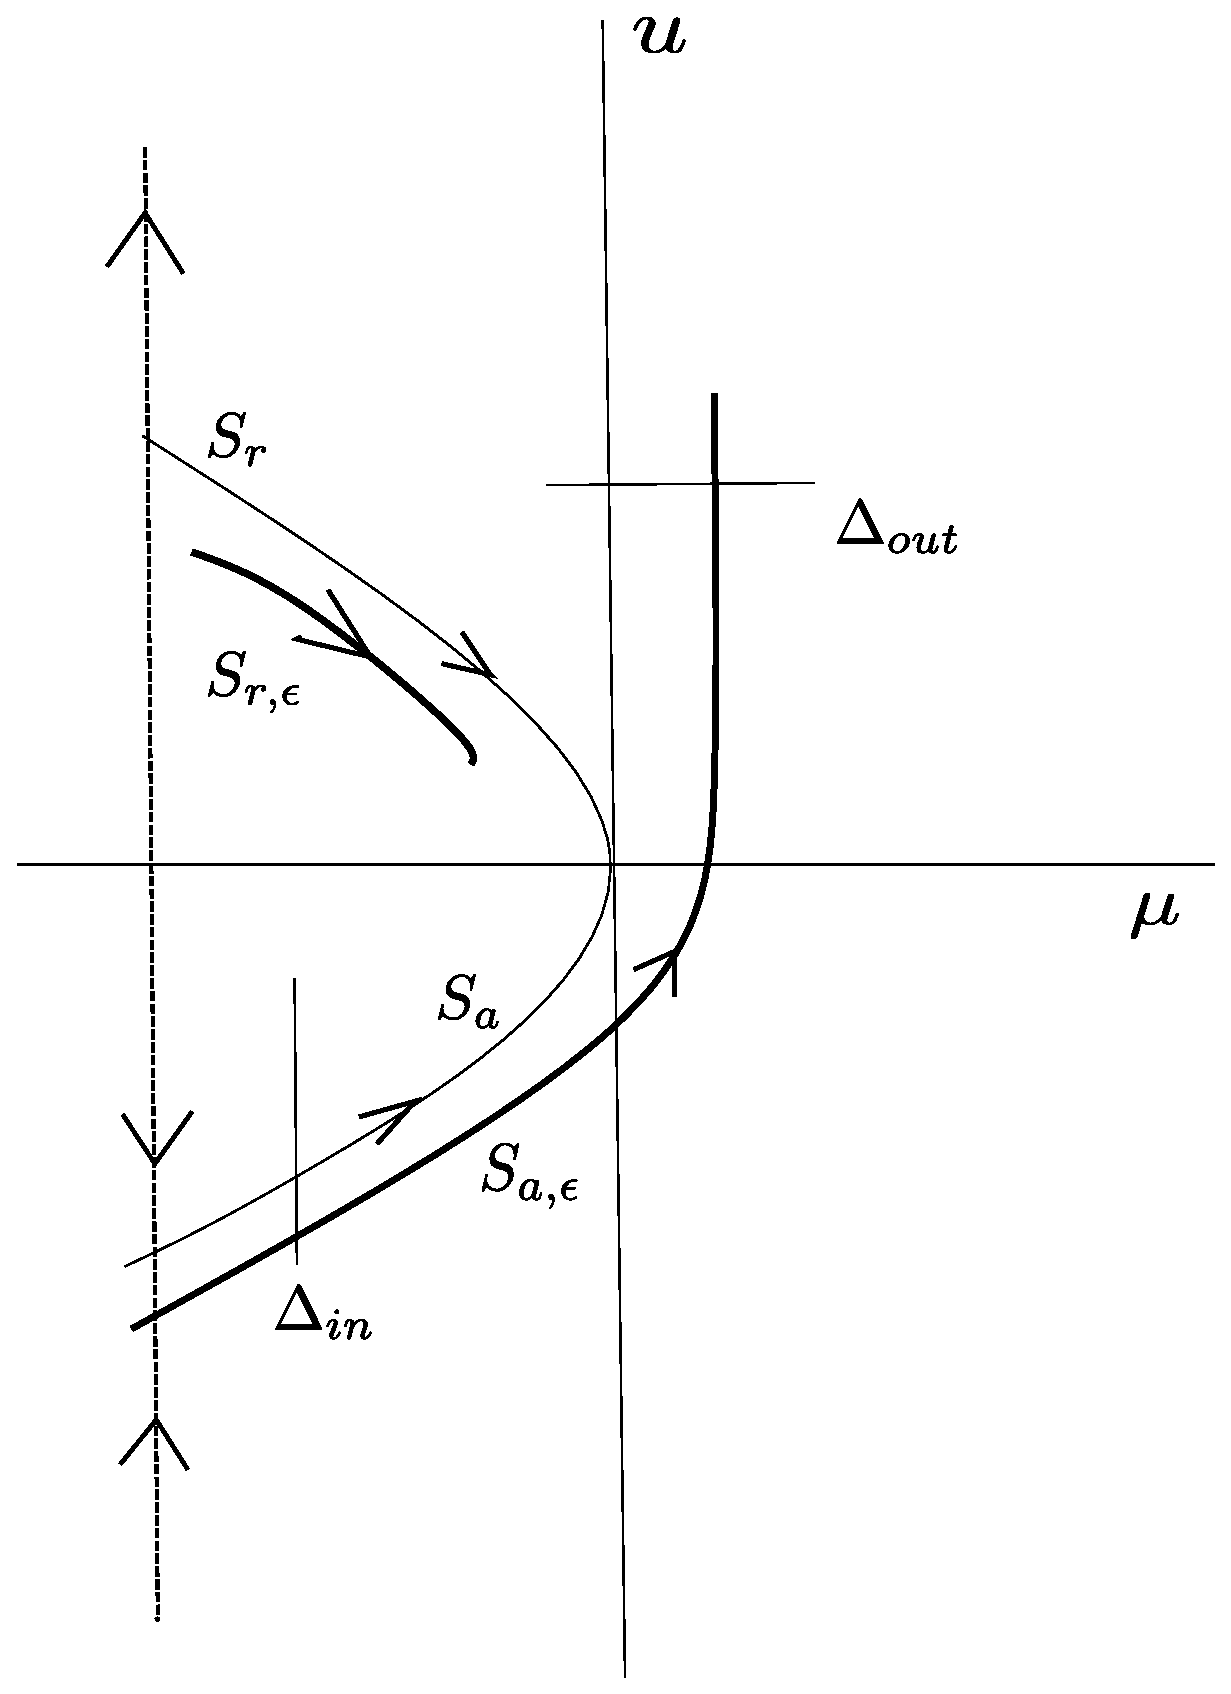
\includegraphics{figures/passage_fold.eps}} % importing figure
 \caption{critical manifold and slow manifolds, section near the fold\label{fig:passage}}
\end{figure}

 Away from the fold point $(0,0,0)$, there exist the attracting manifold $M_a$ with a section $S_a$ sketched in Figure \ref{fig:passage}. By standard Fenichel's theory, $S_a$ perturbs to $S_{a,\eps}$ until it reaches the fold point, thus a natural question is to track how a trajectory starting on the slow manifold $S_{a,\eps}$ passes through the fold point.

For a small interval $J$ containing $-\sqrt{\delta}$, Krupa and Szmolyan starts by setting two sections $\Delta_{in} = \{(-\delta, u) : u \in J \}$ and $\Delta_{out} = \{( \mu ,\sqrt{\delta}): \mu \in \mathbb{R})\}$ with $\delta>0$ small but fixed, which are also shown in figure \ref{fig:passage}. To track the passage through the fold amounts to study the transition map 
\[
\pi: \Delta_{in} \to \Delta_{out},
\]

Krupa and Szmolyan then proceed by defining the blow up transformation
\[
u =\bar{r} \bar{u},  \quad \mu = \bar{r}^2 \bar{\mu}, \quad  \eps = \bar{r}^3 \bar{\eps},
\]
which ``blows up'' the vector field of the extended $(\mu, u, \eps)$ system near $(0,0,0)$ into a vector field on the ball $B = S^2 \times [0,\eps_0^{1/3}] \ni (\bar{u}, \bar{\mu}, \bar{\eps}, \bar{r})$ for some $\eps_0>0$ small, and further directional blow-ups to obtain charts $K_1,K_2,K_3$ which was used to describe the flows in regions near different parts of the manifold $B$. After a careful and thorough analysis, they were able to prove the following results:
\begin{Theorem}\label{ks_main}(Theorem 2.1 in \cite{KrupaSz})

For $\eps$ sufficiently small, the following statements are true:
\begin{enumerate}
\item The manifold $S_{a,\eps} $ passes through  $\Delta_{out}$ at a point $(h(\eps), \sqrt{\delta})$ where $h(\eps) = \rmO(\eps^{2/3})$.
\item The transition map $\pi$ is a contraction with rate $\rmO(e^{-c/\eps} )$, where $c$ is a positive constant independent of $\eps$.
\end{enumerate}
\end{Theorem}


In this paper, we focus on the same problem \eqref{ori_eqn} with an aim to recreate the result of Theorem \ref{ks_main} via a different, functional-analytical approach. Instead of proceeding with the geometrically-flavored blow-up approach, we directly prove a trajectory exists with the properties claimed in Theorem \ref{ks_main} by dividing the time of passage into appropriate parts and setting up a corresponding ansatz in each region, closing the arguments with carefully reformulating the existence question as a fixed-point argument.

To summarize, we first make a change of variable to transform \eqref{ori_eqn} into a more convenient form in Section \ref{euler_m}. Then we introduces the different ansatz used in Section \ref{Ric_def} and \ref{c_mfld}. We then give a statement of our main result in Section \ref{main_sum}.
\subsection{Euler multiplier}\label{euler_m}
Let $\tau$ denote the independent time variable in \eqref{ori_eqn}, since for $u,\mu,\eps$ small, $g(u,\mu,\eps) = 1 + \rmO(u,\mu,\eps)>0$, we can define a new time $t = t(\tau)$ by $\frac{dt}{d\tau} = g$, consequently, \eqref{ori_eqn}  is transformed into
\begin{align}\label{euler_ori_eqn}
\begin{split}
\frac{d}{dt}u &= \mu+u^2+ \tilde{f}(u,\mu;\eps),\\
\frac{d}{dt}\mu &=  \eps ,
\end{split}
\end{align}
where now $\tilde{f}$ satisfies the asymptotics
\begin{equation}\label{nonlinear_asy_new}
\tilde{f}(u,\mu,\eps) = \rmO(\eps,  u\mu, \mu^2,\eps u, \eps \mu, \eps u^2, u^3).
\end{equation}  

The critical manifold 
\[
\tilde{S}_0 = \{ (\mu, u) \mid \mu + u^2 + \tilde{f}(u,\mu;0) = 0\},
\]
still has $(0,0,0)$ as the only fold point, and our goal is to track how a trajectory of the flow of \eqref{euler_ori_eqn} passes through the fold. Following the set up of the sections $\Delta_{in}$ and $\Delta_{out}$ in Krupa-Szmolyan, we propose the following boundary conditions

\begin{equation}\label{ori_bc}
\mu(0) = -\delta_-, \hspace{0.2in} u(T) = \delta_+,
\end{equation}
where $T$ is also an unknown variable which marks the ``time of exit'' as the trajectory hits the section $\Delta_{out}$, and $\delta_{\pm}$ are small positive numbers.

That is, we think the tracking of the passage of the fold as a shooting problem, if we can prove the existence of a solution $(\mu, u)$ to \eqref{euler_ori_eqn} with the boundary condition \eqref{ori_bc}, and give the expansion for the components $\mu$, then we will prove the results in \eqref{ori_eqn}. Our contribution in this paper is that the method we used to prove the existence of such a solution is different than the blow-up approach.

In the rest of the paper, we shall drop the tilde to use $f(u,\mu,\eps)$ as the nonlinearity and $S_0$ to denote the critical manifold.



\subsection{The Riccati equation}\label{Ric_def}
First, we want to get an idea of what kinds of ansatz one should use. Consider \eqref{euler_ori_eqn} with $f(u,\mu;\eps) = 0$, which can then be scaled such that $\eps = 1, \mu = s$, and 
\begin{equation}\label{ric}
\frac{d}{ds}u(s) = s+u(s)^2,
\end{equation}

which is the Ricatti equation in its simplest form. We denote any solution to \eqref{ric} as $u_R$, it is known to have a unique solution (denoted by $\bar{u}_R$) with the following asymptotic expansions (see \cite{KrupaSz} as well).

\begin{equation} \label{ric_asy}
\bar{u}_R(s)=\begin{cases}
  (\Omega_0-s)^{-1}+\rmO(\Omega_0-s), \text{ as }s \to \Omega_0, \\
 -(-s)^{1/2} -\frac{1}{4}(-s)^{-1} + \rmO(|s|^{-3/2}), \text{ as }s \to -\infty.
\end{cases}
\end{equation}

Here the constant $\Omega_0 \approx 2.3381$ is the smallest positive zero of 
\[
J_{-1/3}(2z^{3/2}/3)+J_{1/3}(2z^{3/2}/3),
\]
where $J_{\pm 1/3}$ are Bessel functions of the first kind.


More generally, we consider family of solutions  $u_R(s; u_0)$ of the Riccati equation  \eqref{ric} such that $u_R(0; u_0) = u_0$. That is, we take the initial condition $u_0$ as a parameter to the Riccati equation. For the special Riccati solution $\bar{u}_R$, we define
\begin{equation}\label{def:bar_u_0}
 \bar{u}_0:= \bar{u}_R(0).
\end{equation} 
In fact, using simple phase plane analysis, we can extend the asymptotic results about the special Riccati solution $\bar{u}_R$ to the family of solutions $u_R(s; u_0)$ as follows.

\begin{Proposition}\label{para_ric}
There exist $\eta>0$ small, so that for all initial condition $u_0$ with $|u_0- \bar{u}_0|<\eta$, there exist a number $\Omega_\infty=\Omega_\infty(u_0)$ which depends on $u_0$ smoothly, and a solution $u_R(s;u_0)$ of \eqref{ric} on $[0, \Omega_\infty)$ with the following asymptotic expansion as $s\to \Omega_\infty$:
\begin{equation}\label{ric_exp}
u_R(s;u_0) = \frac{1}{\Omega_\infty-s} +  (\Omega_\infty-s) r(\Omega_\infty-s;u_0),
\end{equation}
where the function $r$ is smooth in both variables and satisfies
\begin{equation}\label{ric_reminder}
r( \Omega_\infty-s; u_0) = -\frac{\Omega_\infty}{3} + \rmO(\Omega_\infty-s),
\end{equation}
as $s \to \Omega_\infty$.
\end{Proposition}
We postpone the proof of this proposition to the appendix.

\subsection{Critical manifold}\label{c_mfld}
Another piece of the ansatz comes from part of  the critical manifold, we expect this because away from the fold, the critical manifold has an attracting branch $S_a$ which implies trajectory has to stay close to it. 

Recall the critical manifold for \eqref{crit_mfld} is the set of points $(\mu, u) $ in a small neighborhood of the origin which satisfies
\begin{equation} \label{crit_mfld}
\mu + u^2 + f(u,\mu; 0) =  0.
\end{equation}

From \eqref{nonlinear_asy_new} we see that $\mu = -u^2+\rmO(u^3)$, by rescaling $\mu = -\mu_1^2$ with $\mu_1$ positive and $u=\mu_1 u_1$ we obtain
\[
u_1^2 = 1 + \rmO(\mu_1),
\]
and hence two branches of solutions
\[
u_1 = \pm \sqrt{1}+\rmO(\mu_1) \implies u = \pm \sqrt{-\mu}+\rmO(\mu).
\]

We therefore define
\begin{align}
\begin{split}
u_-(\mu) &= -\sqrt{-\mu} + \rmO(|\mu|),\\
u_+(\mu) &= +\sqrt{-\mu} + \rmO(|\mu|).
\end{split}
\end{align}


In particular, we set
\begin{equation}\label{singular}
u_s(t)=u_-(\mu(t)) ,
\end{equation}
so that
\[
0 = \mu(t) + u_s^2(t)+f(u_s(t),\mu; 0).
\]
Due to the simple form of \eqref{euler_ori_eqn} and \eqref{ori_bc}, we have that $\mu(t)= \eps t-\delta_-$, hence $u_s(\mu)$ satisfies
\begin{equation}\label{singularAsy}
u_s(t) = -\sqrt{\delta-\eps t} + \rmO(|\delta-\eps t|).
\end{equation}


\subsection{Main result - summary} \label{main_sum}

We now state our main result. Recall $\mathcal{U}$ is a neighborhood small enough so that \eqref{fold_nonlinearity} holds for $(\mu, u , \eps) \in \mathcal{U}$.

\begin{Theorem}[passage through fold]\label{thm:main}Let $\Omega_0$ be the constant defined in \eqref{ric_asy}.
Fix $\delta_-, \delta_+>0$ and $\alpha$ with $0<\alpha <3/4$. There exist $\eps_0>0,$ a constant $C=C(\delta,\alpha),$ such that for all $0<\eps<\eps_0$ and $u_i$ with $|u_i -u_-(-\delta) | \le C\eps^{1-\alpha/3}$, a solution of the rescaled system 
\begin{equation}\label{main_eqn}
\begin{split}
\frac{d}{dt}u &= \mu+u^2+ f(u,\mu;\eps), \\
\frac{d}{dt} \mu &= \eps.  \\
\end{split}
\end{equation}
with the initial condition
\begin{equation}\label{main_ic}
\begin{split}
u(0) &= u_i, \\
\mu(0) &= -\delta_-,
\end{split}
\end{equation}

exists for $t \in (0,T)$, where the end point $T$ is the desired ``exit time'' in the sense that 
\begin{equation}\label{exit_time_cond}
 u(T) = \delta_+.
\end{equation}

Moreover, $T$ has the following expansion in $\eps$
\begin{equation}\label{T_exp_+}
T = T(\eps ; u_i) = \eps^{-1}\delta_- + \eps^{-1/3}\Omega_0 +  \mathcal{H}(\eps; u_i),
\end{equation}
with the term $\mathcal{H}(\eps;u_i)$ satisfies 
\begin{equation}\label{T_remainder_exp}
\eps\mathcal{H}(\eps;u_i) = \rmO(\eps^{1-\alpha/3}), \hspace{0.2in} \text{Lip}_{u_i}\eps\mathcal{H}(\eps;u_i) = \rmO(1).
\end{equation}
In particular, since $\mu(t) = \eps t -\delta_-$, we have the following expansion of the exit location $\mu(T)$ on the section $\Delta_{out}$ in $\eps$:
\begin{equation}\label{exit_loc_exp}
\mu(T) = \eps^{2/3}\Omega_0  + \eps\mathcal{H}(\eps; u_i) = \eps^{2/3}\Omega_0 + \rmO(\eps^{1-\alpha/3}).
\end{equation}

\end{Theorem}

To fully recover Theorem \ref{ks_main}, we have the following corollary.
\begin{Corollary}\label{cor:main}
For $\alpha,\delta_-,\delta_+>0$, there is a compact interval $K \subset (-\infty, u_+(-\delta_-))$, independent of $\eps$ so that for all $u_i \in K$ with $(u_i,\mu,\eps) \in \mathcal{U}$, the same conclusion of Theorem \ref{thm:main} holds. In fact, there exist a constant $c$ independent of $\eps$, such that the Lipschitz constant of $\mathcal{H}(\eps;u_i)$ in the expansion \eqref{T_exp_+} satisfies
\begin{equation}\label{T_remainder_exp_+}
\text{Lip}_{u_i} \eps\mathcal{H}(\eps;u_i) = \rmO(e^{-c/\eps}),
\end{equation}
for all $u_i \in K$.
\end{Corollary}



\textbf{Remark:} Notice $\alpha>0$ could be chosen arbitrary small in the expansion \eqref{exit_loc_exp}. In fact, it is well-known from the matched-asymptotics community that the next order term after $\eps^{2/3}\Omega_0$ is of order $\eps \log(\eps)$.  This is also confirmed in \cite{KrupaSz} using the blow-up methods. 